\documentclass{article}
\usepackage{amsmath}
\usepackage{amssymb}
\usepackage{tikz}
\usepackage{pgfplots}
\pgfplotsset{compat=1.16}

\begin{document}

\begin{figure}[h]
    \centering
    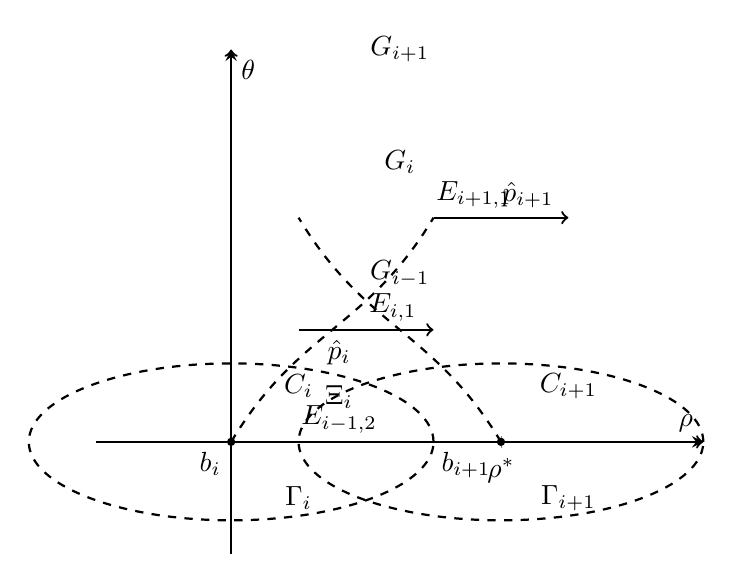
\begin{tikzpicture}
        \begin{axis}[
            axis lines = center,
            xlabel = $\rho$,
            ylabel = {$\theta$},
            xmin=-0.5, xmax=3.5,
            ymin=-0.5, ymax=3.5,
            xtick={-1, 2}, ytick={0},
            xticklabels={$-\rho^*$, $\rho^*$},
            yticklabels={},
            domain=-0.5:3.5,
            samples=100,
            smooth,
            no markers,
            thick,
            every axis plot/.append style={line width=1pt},
            clip=false,
            ]
            
            % Ellipses
            \draw[dashed] (0,0) ellipse [x radius=1.5, y radius=0.7];
            \draw[dashed] (2,0) ellipse [x radius=1.5, y radius=0.7];
            
            % Lines
            \draw[->] (-1,0) -- (3.5,0);
            \draw[->] (0,-1) -- (0,3.5);
            
            % Labels
            \node at (0.5, 0.5) {$C_i$};
            \node at (2.5, 0.5) {$C_{i+1}$};
            
            % Points
            \fill (0,0) circle (1.5pt) node[below left] {$b_i$};
            \fill (2,0) circle (1.5pt) node[below left] {$b_{i+1}$};
            
            % Curves
            \draw[thick, dashed] (0,0) .. controls (0.5,1) and (1,1) .. (1.5,2);
            \draw[thick, dashed] (2,0) .. controls (1.5,1) and (1,1) .. (0.5,2);
            
            % Labels for curves
            \node at (1.25, 1.5) {$G_{i-1}$};
            \node at (1.25, 2.5) {$G_i$};
            \node at (1.25, 3.5) {$G_{i+1}$};
            
            % Labels for points on curves
            \node at (0.8, 0.8) {$\hat{p}_i$};
            \node at (2.2, 2.2) {$\hat{p}_{i+1}$};
            
            % Labels for intersections
            \node at (0.8, 0.2) {$E_{i-1,2}$};
            \node at (1.2, 1.2) {$E_{i,1}$};
            \node at (1.8, 2.2) {$E_{i+1,1}$};
            
            % Labels for ellipses
            \node at (0.5, -0.5) {$\Gamma_i$};
            \node at (2.5, -0.5) {$\Gamma_{i+1}$};
            
            % Labels for intersection points
            \node at (0.8, 0.4) {$\Xi_i$};
            
            % Arrows
            \draw[->] (1.5, 2) -- (2.5, 2);
            \draw[->] (0.5, 1) -- (1.5, 1);
            
        \end{axis}
    \end{tikzpicture}
    \caption{Geometrical Visualization of the construction in the proof of Theorem \ref{thm:elliptic_decomposition} for the case where $b_i$ is repelling and $b_{i+1}$ is attracting.}
    \label{fig:elliptic_decomposition}
\end{figure}

\end{document}